\documentclass[letterpaper, 10pt, titlepage, twocolumn]{article}
\usepackage{graphicx}
\usepackage{authblk}
\usepackage{biblatex}
\usepackage{titling}
\usepackage{float}
\usepackage[left=1.5cm, right=1.5cm, top=2cm, bottom=2cm]{geometry}
\usepackage{fancyhdr}
\usepackage{multicol}
\usepackage{adjustbox}
\usepackage{tikz}
\usepackage{soul}
%\usepackage[sc]{titlesec}
\graphicspath{{./images/}}
\addbibresource{NNSS.bib}

\usepackage{amsmath}
\tikzset{>=latex} % for LaTeX arrow head
\usepackage{pgfplots} % for the axis environment
\usepackage{xcolor}
\usepackage[outline]{contour} % halo around text
\contourlength{1.2pt}
\usetikzlibrary{positioning,calc}
\usetikzlibrary{backgrounds}% required for 'inner frame sep'
%\usepackage{adjustbox} % add whitespace (trim)

% define gaussian pdf and cdf
\pgfmathdeclarefunction{gauss}{3}{%
  \pgfmathparse{1/(#3*sqrt(2*pi))*exp(-((#1-#2)^2)/(2*#3^2))}%
}
\pgfmathdeclarefunction{cdf}{3}{%
  \pgfmathparse{1/(1+exp(-0.07056*((#1-#2)/#3)^3 - 1.5976*(#1-#2)/#3))}%
}
\pgfmathdeclarefunction{fq}{3}{%
  \pgfmathparse{1/(sqrt(2*pi*#1))*exp(-(sqrt(#1)-#2/#3)^2/2)}%
}
\pgfmathdeclarefunction{fq0}{1}{%
  \pgfmathparse{1/(sqrt(2*pi*#1))*exp(-#1/2)}%
}

\colorlet{mydarkblue}{blue!30!black}
\definecolor{bordergray}{HTML}{CCCCCC}

% to fill an area under function
\usepgfplotslibrary{fillbetween}
\usetikzlibrary{patterns}
\pgfplotsset{compat=1.12} % TikZ coordinates <-> axes coordinates

\def\figurewidth{10cm}
\def\figurewidthalt{6cm}
\def\axisdefaultwidth{\figurewidth}

\def\N{255}
\begin{document}
\begin{titlepage}
    \begin{center}
        \vspace*{1cm}

        \LARGE \textbf{Uncertainty Propagation in Regularization-Based Image Deblurring}

        \vspace{0.5cm}
        \Large Research Project Proposal
        
        \vspace{2.0cm}
        \large \textbf{Thomas Pasfield}

        \vspace{0.5cm}
        As submitted on:\\
        \today

        \vfill

        Supervising Professor:\\
        Dr. Harihar Khanal\\
        \vspace{1em}
        \normalsize Department of Mathematics\\
        Embry-Riddle Aeronautical University\\
        Daytona Beach, FL
    \end{center}
\end{titlepage}
%\maketitle

%\begin{multicols}{2}
\section*{Introduction}
Image blur hinders quantitative image analysis, especially in the field of radiographic imaging. By approaching image deblurring as deconvolution (an ill-posed inverse problem), methods such as Tikhonov and Total Variation Regularization present appropriate solutions. As non-blind deblurring methods, the regularization methods require an estimate or exact measurement of the Point Spread Function (PSF) of the optical system. The PSF is unknown but can be estimated from a calibration image. This estimation process introduces uncertainty into the final solution. In this work, I aim to provide a comprehensive analysis of the uncertainty propagation from the PSF estimate through the regularization processes. The results will provide insight into the deblurring methods already in use, and allow for informed analysis of the deblurred outputs.

Existing work in this application is thoroughly explored by Dr. Jordan Pillow of the Nevada National Security Site in his 2021 PhD Thesis. \cite{pillow_bayesian_2021} % TODO

\section*{Problem Description}
\subsection*{Blur as Convolution}
Performing regularization requires this problem to be approached with traditional computer vision techniques rather than the machine learning techniques that have become more popular. These traditional computer vision techniques often represent operations on images as linear models, which is a practice which will be continued here. Our image, $\mathbf{X}$, is a two-dimensional matrix representing a black-and-white image or a single color channel from a color image, with shape $(m,n)$. The color depth of the image is largely irrelevant. The process of image blurring can be represented as a convolution of the PSF across the image, cropped to the original window of the image. The blurred image is represented by $\mathbf{B}$, which shares the same shape $(m,n)$ of the original image. This system is shown in Equation \eqref{eqn:conv}.

\begin{equation}
    \label{eqn:conv}
    \mathbf{B}=\mathbf{X} \ast \textrm{PSF}
\end{equation}

\subsection*{Creating a Linear Model}
This equation, however, is not a linear model and cannot be used in regularization. It must first be discretized into matrices. When the PSF depends only on the X and Y axes, it can be known as separable blur. Separable blur can be represented by two different convolution operations: one where the kernel only affects the X-axis, and another where the kernel only affects the Y-axis. A 1-D PSF can be represented as a vector along the axis that is being blurred along. For a rather simple system, this 1-D PSF may approximate a Gaussian distribution. This is demonstrated within Figure \ref{tikz:1dkernel}. From this point on, the exact structure used to discretize the convolution is dependent on the boundary conditions applied to the image. In this case, it is certain that there is a zero boundary, so all work from this point forward will use the structures and methods specific to that case. See \emph{Deblurring Images: Matrices, Spectra, and Filtering} \cite{hansen_deblurring_2006} for more information on this structure.

% Tikz Figure of Gaussian Distribution
\begin{figure}[H]
\centering
\begin{tikzpicture}[inner frame sep=0]
  \message{p-value^^J}
  \def\B{0};
  \def\Bs{1.0};
  \def\xmax{\B+16.0*\Bs};
  \def\ymin{{-0.15*gauss(\B,\B,\Bs)}};
  
  \begin{axis}[every axis plot post/.append style={
               mark=none,domain={-0.0001}:{1.08*\xmax},samples=\N,smooth},
               xmin={-0.018*(\xmax)}, xmax=\xmax,
               ymin=\ymin, ymax={1.1*gauss(\B,\B,\Bs)},
               axis lines=middle,
               axis line style=thick,
               enlargelimits=upper, % extend the axes a bit to the right and top
               ticks=none,
               every axis x label/.style={at={(current axis.right of origin)},anchor=north west},
               y=100pt,
              ]
    % PLOTS
    \addplot[name path=B,thick,black!10!blue] {gauss(x,\B,\Bs)};
    % FILL
    \path[name path=xaxis]
      (0,0) -- (\xmax,0);
    \addplot[white!50!blue] fill between[of=xaxis and B, soft clip={domain=0.0:\xmax}];
  \end{axis};
\end{tikzpicture}

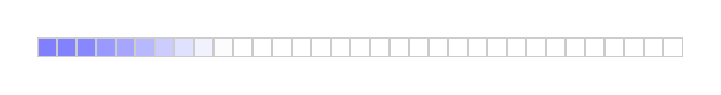
\begin{tikzpicture}
  [nodes=draw,
  column 1/.style={bordergray, nodes={fill=white!50!blue}},
  column 2/.style={bordergray, nodes={fill=white!51!blue}},
  column 3/.style={bordergray, nodes={fill=white!53!blue}},
  column 4/.style={bordergray, nodes={fill=white!60!blue}},
  column 5/.style={bordergray, nodes={fill=white!65!blue}},
  column 6/.style={bordergray, nodes={fill=white!72!blue}},
  column 7/.style={bordergray, nodes={fill=white!80!blue}},
  column 8/.style={bordergray, nodes={fill=white!88!blue}},
  column 9/.style={bordergray, nodes={fill=white!95!blue}},
  column 10/.style={bordergray, nodes={fill=white!99!blue}},
  column 11/.style={bordergray, nodes={fill=white}},
  column 12/.style={bordergray, nodes={fill=white}},
  column 13/.style={bordergray, nodes={fill=white}},
  column 14/.style={bordergray, nodes={fill=white}},
  column 15/.style={bordergray, nodes={fill=white}},
  column 16/.style={bordergray, nodes={fill=white}},
  column 17/.style={bordergray, nodes={fill=white}},
  column 18/.style={bordergray, nodes={fill=white}},
  column 19/.style={bordergray, nodes={fill=white}},
  column 20/.style={bordergray, nodes={fill=white}},
  column 21/.style={bordergray, nodes={fill=white}},
  column 22/.style={bordergray, nodes={fill=white}},
  column 23/.style={bordergray, nodes={fill=white}},
  column 24/.style={bordergray, nodes={fill=white}},
  column 25/.style={bordergray, nodes={fill=white}},
  column 26/.style={bordergray, nodes={fill=white}},
  column 27/.style={bordergray, nodes={fill=white}},
  column 28/.style={bordergray, nodes={fill=white}},
  column 29/.style={bordergray, nodes={fill=white}},
  column 30/.style={bordergray, nodes={fill=white}},
  column 31/.style={bordergray, nodes={fill=white}},
  column 32/.style={bordergray, nodes={fill=white}},
  column 33/.style={bordergray, nodes={fill=white}},
  column 34/.style={bordergray, nodes={fill=white}},
  column 35/.style={bordergray, nodes={fill=white}},
  ]
  \matrix[draw=white]{
    \node {\hspace{1em}}; & \node {\hspace{1em}}; & \node {\hspace{1em}}; & \node {\hspace{1em}}; & \node {\hspace{1em}}; & \node {\hspace{1em}}; & \node {\hspace{1em}}; & \node {\hspace{1em}}; & \node {\hspace{1em}}; & \node {\hspace{1em}}; & \node {\hspace{1em}}; & \node {\hspace{1em}}; & \node {\hspace{1em}}; & \node {\hspace{1em}}; & \node {\hspace{1em}}; & \node {\hspace{1em}}; & \node {\hspace{1em}}; & \node {\hspace{1em}}; & \node {\hspace{1em}}; & \node {\hspace{1em}}; & \node {\hspace{1em}}; & \node {\hspace{1em}}; & \node {\hspace{1em}}; & \node {\hspace{1em}}; & \node {\hspace{1em}}; & \node {\hspace{1em}}; & \node {\hspace{1em}}; & \node {\hspace{1em}}; & \node {\hspace{1em}}; & \node {\hspace{1em}}; & \node {\hspace{1em}}; & \node {\hspace{1em}}; & \node {\hspace{1em}};\\
  };
\end{tikzpicture}

\caption{A plot of a Gaussian distribution PSF and a representation of a corresponding vector to convolve this PSF along the x-axis.}
\label{tikz:1dkernel}
\end{figure}

Convolutions can be discretized quite easily by taking a 1-D kernel and creating a Toeplitz matrix with it. This matrix, when multiplied with the vectorized (column-stacked) image vector, performs a convolution of the kernel along the expected axis. This discretized convolution can be seen in Figure \ref{fig:toeplitz}. More work is required to discretize a 2-D convolution. First, discrete convolution matrices must be generated for both the blur along the x and y axes. Then the 2-D discrete convolution matrix is formed by taking the Kronecker product of the two components. This 2-D convolution matrix is shown within Figure \ref{fig:kronecker}. This 2-D convolution matrix will be represented via \textbf{A}, and its respective components by $\mathbf{A_x}$ and $\mathbf{A_y}$. This new matrix \textbf{A} has a size of ($mn$, $mn$). The convolution is performed by multiplying the convolution matrix with the column-stacked vectorized image matrix. These relationships are all observed in Equations \eqref{eqn:kron} through \eqref{eqn:linmodel}.

% Toeplitz Image
\begin{figure}[H]
  \centering
  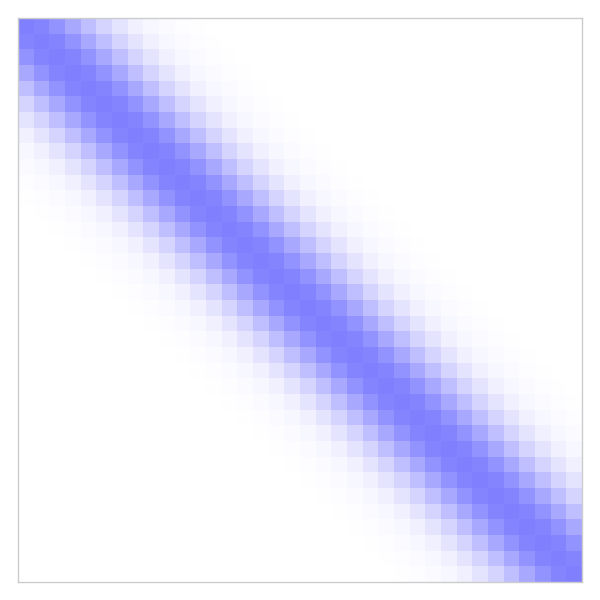
\includegraphics[width=\figurewidthalt]{toeplitz.png}
  \caption{The 1-D PSF extrapolated into a Toeplitz matrix. This matrix now functions as a convolution along the x-axis when multiplied with a vectorized image.}
  \label{fig:toeplitz}
\end{figure}

\begin{equation}
  \label{eqn:kron}
  \mathbf{A} = \mathbf{A_x} \otimes \mathbf{A_y}
\end{equation}

\begin{equation}
  \label{eqn:kronvec}
  \mathbf{B} = \mathbf{A_y}\mathbf{X}\mathbf{A_x}^T
\end{equation}

\begin{equation*}
  \mathbf{b} = \textrm{vec}(\mathbf{B})
\end{equation*}

\begin{equation*}
  \mathbf{x} = \textrm{vec}(\mathbf{X})
\end{equation*}

\begin{equation}
  \label{eqn:linmodel}
  \mathbf{b} = \mathbf{A}\mathbf{x}
\end{equation}

Now that we have these components defined, we can assemble a linear model for an image, seen in Equation \eqref{eqn:fulllinmodel}. This linear model represents a blurred image as a convolution of the PSF across the true image, along with added noise. This added noise can come from various sources, but cannot be modeled on its own. The noise is represented by $\epsilon$, and it takes the shape of a (1, $mn$) vector of normally distribution values. The presence of this noise makes this problem an ill-posed, inverse problem, which invites the regularization methods to follow. 

\begin{equation}
  \label{eqn:fulllinmodel}
  \mathbf{b} = \mathbf{A}\mathbf{x} + \mathbf{\epsilon}
\end{equation}

% Kronecker Product Image
\begin{figure}[H]
  \centering
  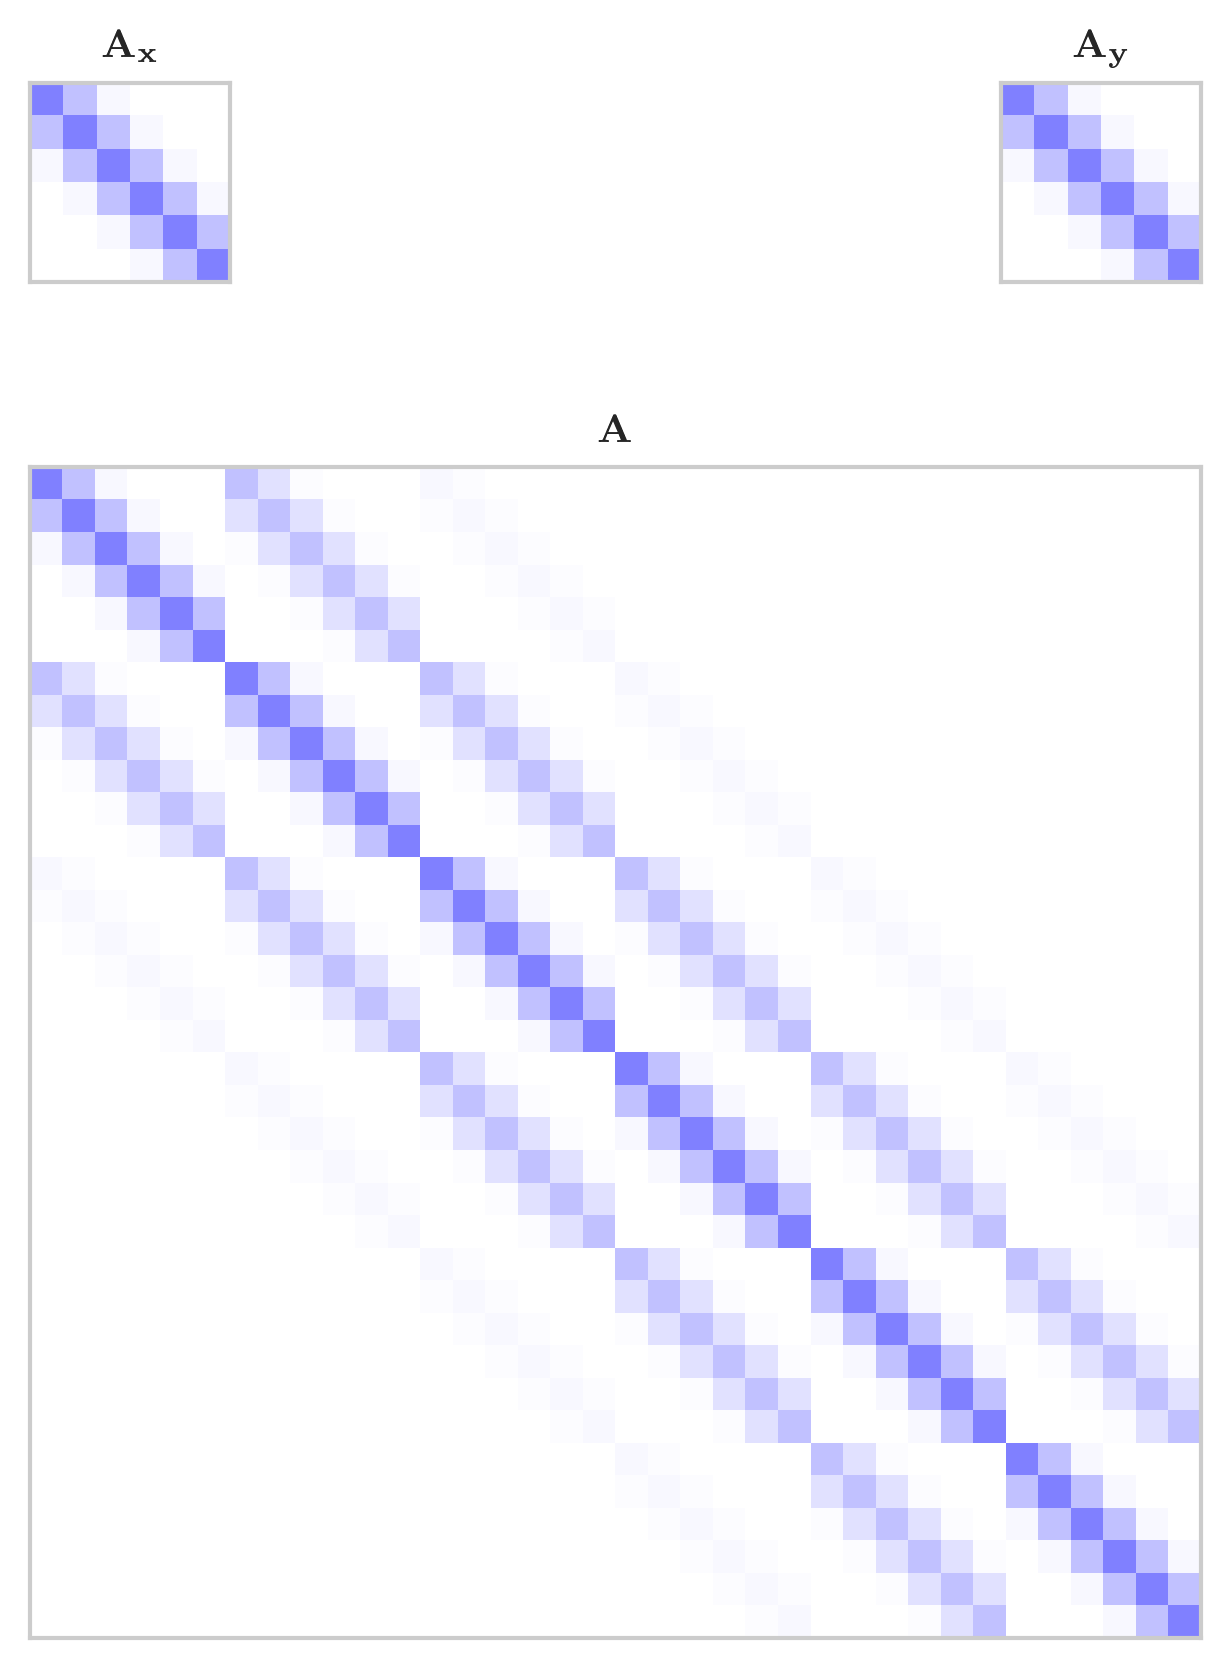
\includegraphics[width=\figurewidthalt]{2dkernel.png}
  \caption{A 2-D discrete convolution matrix formed by performing the Kronecker product of the 1-D discrete convolution matrices.}
  \label{fig:kronecker}
\end{figure}

\subsection*{Regularization}
Regularization is the standard approach to finding plausible solutions for ill-posed inverse problems, and the techniques and strategies are thoroughly described in \emph{Computational Methods for Inverse Problems} \cite{vogel_computational_2002}. Regularization biases an optimization process used to find a possible solution. This bias allows one to tune the output towards an expected property of the solution, such as smoothness.

The two forms of regularization which this work will explore are Tikhonov Regularization, which is also known as L2 or Ridge Regression, and Total Variation Regularization. Tikhonov regularization biases the optimization towards smoother results, while total variation regularization biases results towards blocky results.

\subsubsection*{Tikhonov Regularization}
To bias the optimization towards smooth results, the penalty function attempts to minimize the residuals between the blurred estimate of the solution and the blurred image. This is just a least-squares regression and ensures that the solution maintains some semblance of the blurred image. To make this Tihonov Regularization, the variance is added to the penalty function, which reduces the cost of smoother results compared to noisy or blocky ones. The full optimizer is Equation \eqref{eqn:TIK}. The addition of the Tikhonov factor improves the conditioning of the system, allowing for an explicit form shown in Equation \eqref{eqn:expTIK}. Matrix \textbf{L} is the Tikhonov Matrix, and is simply the identity matrix in this application, while $\alpha$ is a weight parameter that allows for control over how much penalty the variance provides.

\begin{equation}
  \label{eqn:TIK}
  \mathbf{x}_{TIK} = \textrm{argmin}_x\left(||\mathbf{Ax}-\mathbf{b}||^2_2 + \alpha||\mathbf{Lx}||^2_2\right)
\end{equation}

\begin{equation}
  \label{eqn:expTIK}
  = \left(\mathbf{A}^T\mathbf{A} + \alpha \mathbf{L}^T\mathbf{L}\right)^{-1}\mathbf{A}^T\mathbf{b}
\end{equation}

\subsubsection*{Total Variation Regularization}
To bias a solution towards blocky or segmented results, the penalty function must be changed. The base function is still a least-squares solver, as we still need to ensure that the blurred true image is as close to the actual blurred image as possible. Added to the penalty is the weighted Total Variation. This is found using a matrix 1-norm of the product of a discrete derivative operator \textbf{D} with the current image solution. The full optimizer is below in Equation \eqref{eqn:TV}. $\alpha$ shares the same use here as it does with the Tikhonov regularizer.

\begin{equation}
  \label{eqn:TV}
  \mathbf{x}_{TV}=\textrm{argmin}_x\left(\frac{1}{2}||\mathbf{Ax}-\mathbf{b}||^2_2 + \alpha\; ||\mathbf{Dx}||_1\right)
\end{equation}

\subsection*{Parameter Selection}
You may notice that both of these regularization optimizers require a weight parameter $\alpha$. This can be selected arbitrarily by whoever executes the code based on observed changes or prior knowledge, or it can be estimated algorithmically. Algorithmic determination is better suited for this application, though may yield worse results than the user may want, due to ideal outcomes being subjective in nature and difficult to quantify in an optimizer.

Ideally, we could just compare the outcome with an arbitrary parameter to the true image we are solving for, then vary the parameter to minimize residuals. Due to obvious reasons, this is an unrealistic case. We must instead find a reasonably accurate method to predict the error in the solution. This is done via Generalized Cross Validation (GCV).

Unlike typical GCV use, we don't have knowledge of the true image to validate against, but this is easy to work around. We know the blurred image, so we simply blur our solution and compare the blurred solution to the known blurred image. Curtis Vogel \cite{vogel_computational_2002} provides a GCV cost function for Tikhonov regularization, provided in Equation \eqref{eqn:GCVTIK}, where $n$ is dimension stated earlier, and \textbf{F} is an influence matrix defined in Equation \eqref{eqn:influence}. The book provides no derivation of the influence matrix for total variation regularization.

\begin{equation}
  \label{eqn:GCVTIK}
  \textrm{GCV}(\alpha)=\frac{\frac{1}{n}||\mathbf{r}_\alpha||^2}{\left[\frac{1}{n}\;\textrm{trace}(\mathbf{I}-\mathbf{F}_\alpha)\right]^2}
\end{equation}

\begin{equation}
  \label{eqn:influence}
  \mathbf{F}_\alpha = \mathbf{A}\left(\mathbf{A}^T \mathbf{A} + \alpha \mathbf{L}\right)\mathbf{A}^T
\end{equation}

Though there is no derivation for total variation, there are other works which attempt to create a strong GCV cost function for it. Dr. You-Wei Wen of Hunan Normal University \cite{wen_using_2018} derives a GCV function for total variation by finding a representation resembling Tikhonov regularization, then using the known Tikhonov derivation to find the cost. This method will likely be implemented in this work, but that is uncertain.

\section*{Methodology}
Now that we have the foundation of this work laid out, the actual focus of what will be executed must be explained. Within the regularization systems described, all systems rely heavily on the blurring matrix \textbf{A}. If you recall, this matrix is a prediction of what the real blurring process changed, and not a perfect match. This prediction relies on assumptions which may be flawed, and the actual model matching is influenced by noise and randomness within a given observation. We would like to understand how error in this prediction propagates through the regularization and GCV processes to affect the final resolved image.

The calibration process used to predict the blurring matrix is rather simple. To observe blur, we can simply image a line pair (Figure \ref{fig:linepairs}) and measure the value across it, as seen in Figure \ref{fig:esf}. These measurements describe the blur directly, though the noise makes the raw data unsuitable for further work. The PSF must be smooth and continuous, so we must find a smooth, continuous function to match the data. The curve clearly approximates a logistic function, so that is what is used in these examples. Figure \ref{fig:psf} shows how the derivative of this function has the shape of a normal distribution, and thus fits the processes seen in Figure \ref{tikz:1dkernel}. This curve is prepared for the process by simply truncating it to halfway, and padding the end with zeros to achieve the required size, seen in Figure \ref{fig:psfmatrix}. In an ideal scenario, there would be no blur at all and the edge of the line pair would simply be a jump discontinuity to the new value.

\begin{figure}[H]
  \centering
  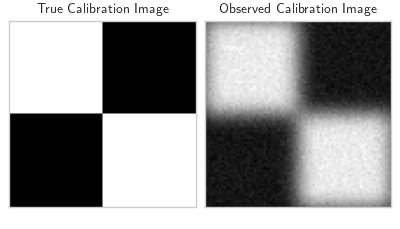
\includegraphics[width=7.5cm]{imgcompare.png}
  \caption{A side-by-side comparison of the true line pair calibration image, containing jump discontinuities from high to low values along both the x and y axes, with the observed result. Note that the observed result is blurred, has considerable noise, and has lost contrast.}
  \label{fig:linepairs}
\end{figure}

\begin{figure}[H]
  \centering
  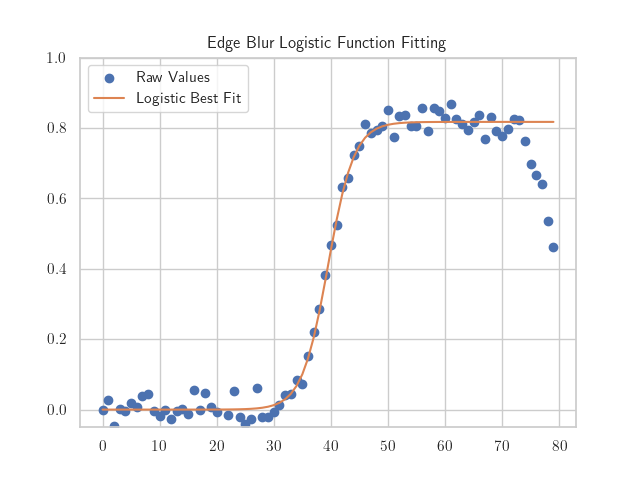
\includegraphics[width=8cm]{edgefit.png}
  \caption{The values across a single row of pixels from the blurred image seen in Figure \ref{fig:linepairs}. The raw values are noisy but follow a logistic function, so a logistic function has been fit to the data.}
  \label{fig:esf}
\end{figure}

The noise alters the residuals when performing the curve fitting, leading to uncertainty in what the real blur is. Due to this, one can curve fit in a manner which gives a lower and upper bound on values which produce a solution with the residual beneath some arbitrary threshold. Sampling can be performed within that range, and the resulting curve can be used for the regularization process. There may be a way to use the Signal-To-Noise ratio to be able to quantify the confidence of how well the curve fit may match the real blur performed.

This problem takes the form of forward propagation of uncertainty, and will consist of taking samples and propagating them through the models to compare the results. Ironically, such a complex foundation of the work has ended up resulting in a rather simple practice in descriptive statistics in the end. 

\begin{figure}[H]
  \centering
  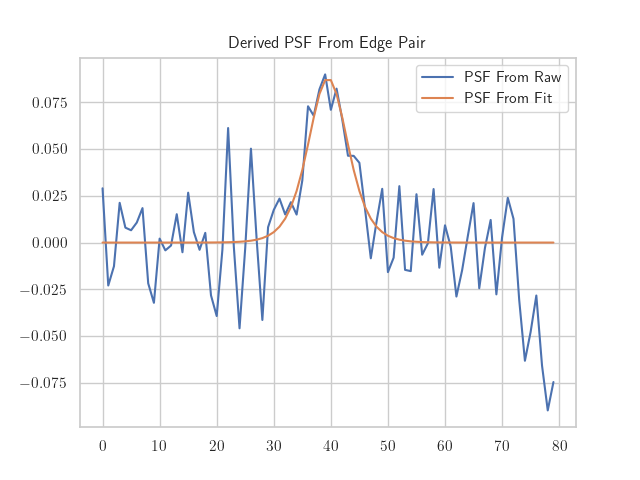
\includegraphics[width=8cm]{derivedpsf.png}
  \caption{The discrete derivative values of both the raw values and the logistic best fit, showing a smooth continuous normal-like function from the logistic curve, and effectively random noise from the raw values. This highlights the importance of the curve fit.}
  \label{fig:psf}
\end{figure}

\begin{figure}[H]
  \centering
  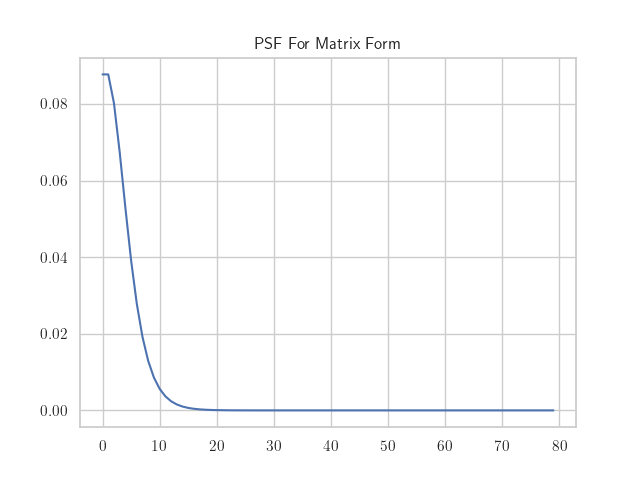
\includegraphics[width=8cm]{matrixpsf.png}
  \caption{The truncated derivative curve, normalized to a sum of 0.5, such that it can be used to create the blurring matrix in the process initially described in Figure \ref{tikz:1dkernel}.}
  \label{fig:psfmatrix}
\end{figure}

To conduct this forward propagation, curve fitting will be performed to determine the best fit. The curve will fit to several rows of the calibration image, rather than just one, to attempt to reduce the effect of noise. Based on the initial solution, Monte Carlo sampling allows for sampling around the parameter. Normally-distributed samples should work well. Each sample will be processed, and the discrete convolution matrix generated.

Initial plans for the computation consist of the following:

\begin{enumerate}
  \item Assign a sampled parameter to two threads from a set of worker threads.
  \item Each parameter is run through the Tikhonov and Total Variation regularizers.\\
    \begin{itemize}
      \vspace*{-0.5em}
      \item Tikhonov regularization is fairly easy to accelerate with Numexpr or Numba.
      \item Total Variation is more complex, but can be distributed with PyLOPs, and PyLOPs-MPI.
    \end{itemize}
  \item Results are aggregated, new workers are deployed until all samples return results.
  \item Solution images will be stacked into a tensor, with statistics computed along the new axis element-wise, such as standard deviation.
\end{enumerate}

\section*{Deliverables}
\begin{itemize}
  \item \normalsize \st{Topic Submission} \footnotesize Due September 20th
  \item \normalsize \st{Project Proposal} \footnotesize Due October 28th
  \item \normalsize Preliminary Report/Presentation \footnotesize Due November 18th
  \item \normalsize Rough Draft \footnotesize Due December 2nd
  \item \normalsize Final Report \footnotesize Due December 9th
\end{itemize}

%\nocite{*}
\printbibliography

%\end{multicols}
\end{document}